\documentclass[border=10pt]{standalone}
\usepackage{amsmath}
\usepackage{tikz}
\usetikzlibrary{positioning, arrows.meta, calc, fit, backgrounds, shapes.geometric}
\begin{document}
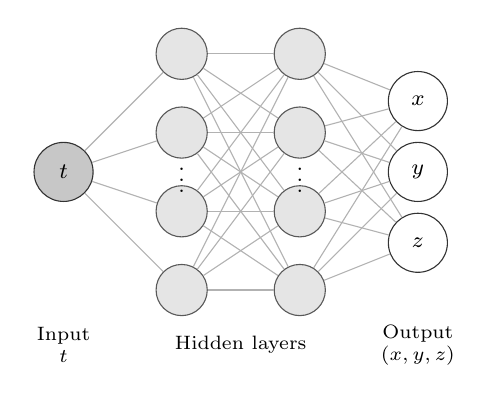
\begin{tikzpicture}[
    font=\footnotesize,
    neuron/.style={circle, draw=black!65, fill=black!10, minimum size=6.5mm, inner sep=0pt},
    inn/.style={circle, draw=black!80, fill=black!22, minimum size=7.5mm, inner sep=0pt},
    outn/.style={circle, draw=black!80, fill=white, minimum size=7.5mm, inner sep=0pt},
    conn/.style={draw=black!30, line width=0.4pt}
]
% input
\node[inn] (i1) at (0,0) {$t$};
% hidden layer A
\foreach \i/\y in {1/1.5,2/0.5,3/-0.5,4/-1.5}{\node[neuron] (a\i) at (1.5,\y) {};}
\node at (1.5,0) {$\vdots$};
% hidden layer B
\foreach \i/\y in {1/1.5,2/0.5,3/-0.5,4/-1.5}{\node[neuron] (b\i) at (3.0,\y) {};}
\node at (3.0,0) {$\vdots$};
% output
\node[outn] (o1) at (4.5, 0.9) {$x$};
\node[outn] (o2) at (4.5, 0.0) {$y$};
\node[outn] (o3) at (4.5,-0.9) {$z$};
% connections
\foreach \i in {1,2,3,4}{\draw[conn] (i1)--(a\i);}
\foreach \i in {1,2,3,4}{\foreach \j in {1,2,3,4}{\draw[conn] (a\i)--(b\j);}}
\foreach \i in {1,2,3,4}{\foreach \o in {o1,o2,o3}{\draw[conn] (b\i)--(\o);}}
% layer captions
\node[align=center, font=\scriptsize] at (0,-2.2) {Input\\$t$};
\node[align=center, font=\scriptsize] at (2.25,-2.2) {Hidden layers};
\node[align=center, font=\scriptsize] at (4.5,-2.2) {Output\\$(x,y,z)$};
\end{tikzpicture}
\end{document}
